\section{簡介}
本章節以及下一個章節將對於問答系統介紹。在過去,閱讀理解和問答系統已經有很多研究提出模型,如加入專注式機制(Attention Mechanism)或急躁機制(Impatient Mechanism)的模型 \cite{hermann2015teaching} ,試圖想要模仿人類的行為,能忽視其他不重要或無關的輸入,只選擇專注於和需求有關的輸入,此方法最早在視覺圖像領域所提出,目的是希望讓機器學到圖片中所應該專注的物件(Object)或位置,而其成效也已經在圖像領域和機器翻譯中得到證實,如 \cite{mnih2014recurrent} 和 \cite{bahdanau2014neural},另有加入了記憶(Memory)網路的 Memory Network \cite{weston2014memory} ,可以儲存理解之後的資訊,概念如同 RNN cell 一般,還有端對端記憶網路(End to End Memory Network)\cite{sukhbaatar2015end} ,透過使用回顧式的機制,來多次更新記憶。本篇論文使用了專注式機制,來選擇文本的哪些部分該注意,使用記憶網路來儲存相關的文本,並且透過回顧式機制來不斷更新記憶網路。

我們可將整個問答系統分成三個部分,首先針對使用者的查詢詞,透過檢索的方式回傳符合查詢詞的文本,但由於回傳的文本過多,因此我們需要一個過濾器(Filter)來判別此文本是否有此查詢詞之答案,以便降低文本的數量。最後在將這些被選出文本與其查詢詞,通過專注式記憶編碼解碼器(Attention-based Memory RNN Encoder-Decoder)\cite{xiong2016dynamic} 抽取出可能的答案,進而回傳給使用者。本論文之研究的檢索部分是採用 Bing 搜尋來取得相關之文本,故僅針對過濾器以及專注式記憶編碼解碼器兩者進行詳細介紹。

在詳細描述模型以前,我們將先簡介機器閱讀理解數據集。 Microsoft 釋出了閱讀理解相關的數據集,而以問答系統來實踐閱讀理解的概念。此數據集約莫有 10 萬筆的問答句以及約 20 萬以上的文章數,對於每個問句,都會有標註此問句的種類,如: cost to get a patent 是被分類為數值(Numeric)、 was ronald reagan a democrat 則是歸類成描述(Description)、diseases caused by clostridium 被歸為名詞(entity)、who was the president who caused the trail of tears 是為人物(Person),而 what sea is iceland in 則為地點(Location)等 5 類,表(\ref{table:query_percentage})和表(\ref{table:query_type})為機器閱讀理解查詢詞之比例。而 Bing 搜尋針對此問句,會提供大約 8 到 10 個左右的文本段落(Passages),人們再根據這些段落,標註此段落「是否」足夠提供問句之答案,並根據段落給予對應一至多個對應的答案。

\begin{table}
    \caption{問句包含詞比例}
    \label{table:query_percentage}
    \centering
    \begin{tabular}[h]{|l|l|}
        \hline
        問句包含詞  &百分比\\
        \hline
        what        &42.2\%\\
        \hline
        how         &15.3\%\\
        \hline
        where       &4.4\%\\
        \hline
        when        &2.0\%\\
        \hline
        why         &1.8\%\\
        \hline
        who         &1.7\%\\
        \hline
        which       &1.4\%\\
        \hline
    \end{tabular}
\end{table}
\begin{table}
    \caption{答案種類}
    \label{table:query_type}
    \centering
    \begin{tabular}{|l|l|}
        \hline
        問句類型            &百分比\\
        \hline
        描述(Description) &52.6\%\\
        \hline
        數字(Numberic)    &28.4\%\\
        \hline
        名詞(Entity)      &10.5\%\\
        \hline
        地點(Location)    &5.7\%\\
        \hline
        人物(Person)      &2.7\%\\
        \hline
    \end{tabular}
\end{table}

\section{模型架構介紹}
%\subsection{專注式記憶編碼解碼器}
圖(\ref{fig:dmn})為本章節之系統架構圖之一。以下會針對此架構圖做分析。

\subsubsection{位置編碼}
首先每個段落透過 Natural Language Toolkit (NLTK)來做英文句子的斷句,即會得到 $M$ 個句子,每個詞都有一個詞向量 $w_j^i$,其中 $i$ 代表第 $i$ 個句子,而 $j$ 代表第 $i$ 個句子的第 $j$ 個詞,一個句子可以使用 RNN ,或者是詞袋模型(Bag of Word Model, BOW)來將編碼(Encode)成一個句向量(Sentence Vector),而此處則是採用位置編碼(Position Encoding)\cite{sukhbaatar2015end}  ,如式子(\ref{PE}),此處使用位置編碼的原因,一方面若是使用詞袋模型,會少了每個詞在句子上順序的重要性,另一方面,使用 RNN 模型雖然能夠有順序之別,但由於本篇論文模型過於複雜,若是使用 RNN 模型,將會有兩層 RNN 來處理詞彙與句子,因此會容易過度貼合,因此本篇論文採取折衷的方法,是採用位置編碼,可以得到每個句子的句向量 $f_i$ 代表第 $i$ 個句子

\begin{equation}
    f_i = \sum_{j=1}^M l_j \circ w_j^i
\end{equation}
其中 $\circ$ 為逐點乘積,而 $l_j$ 則為
\begin{equation}
    l_{jd} = (1 - \frac{j}{M}) - (\frac{d}{D})(1 - \frac{2j}{M}) \label{PE}
\end{equation}
其中 $d$ 是詞向量的第 $d$ 維, $D$ 是詞向量的維度,$j$ 代表一句話的第 $j$ 個詞。

\begin{figure}[h]
    \centering
    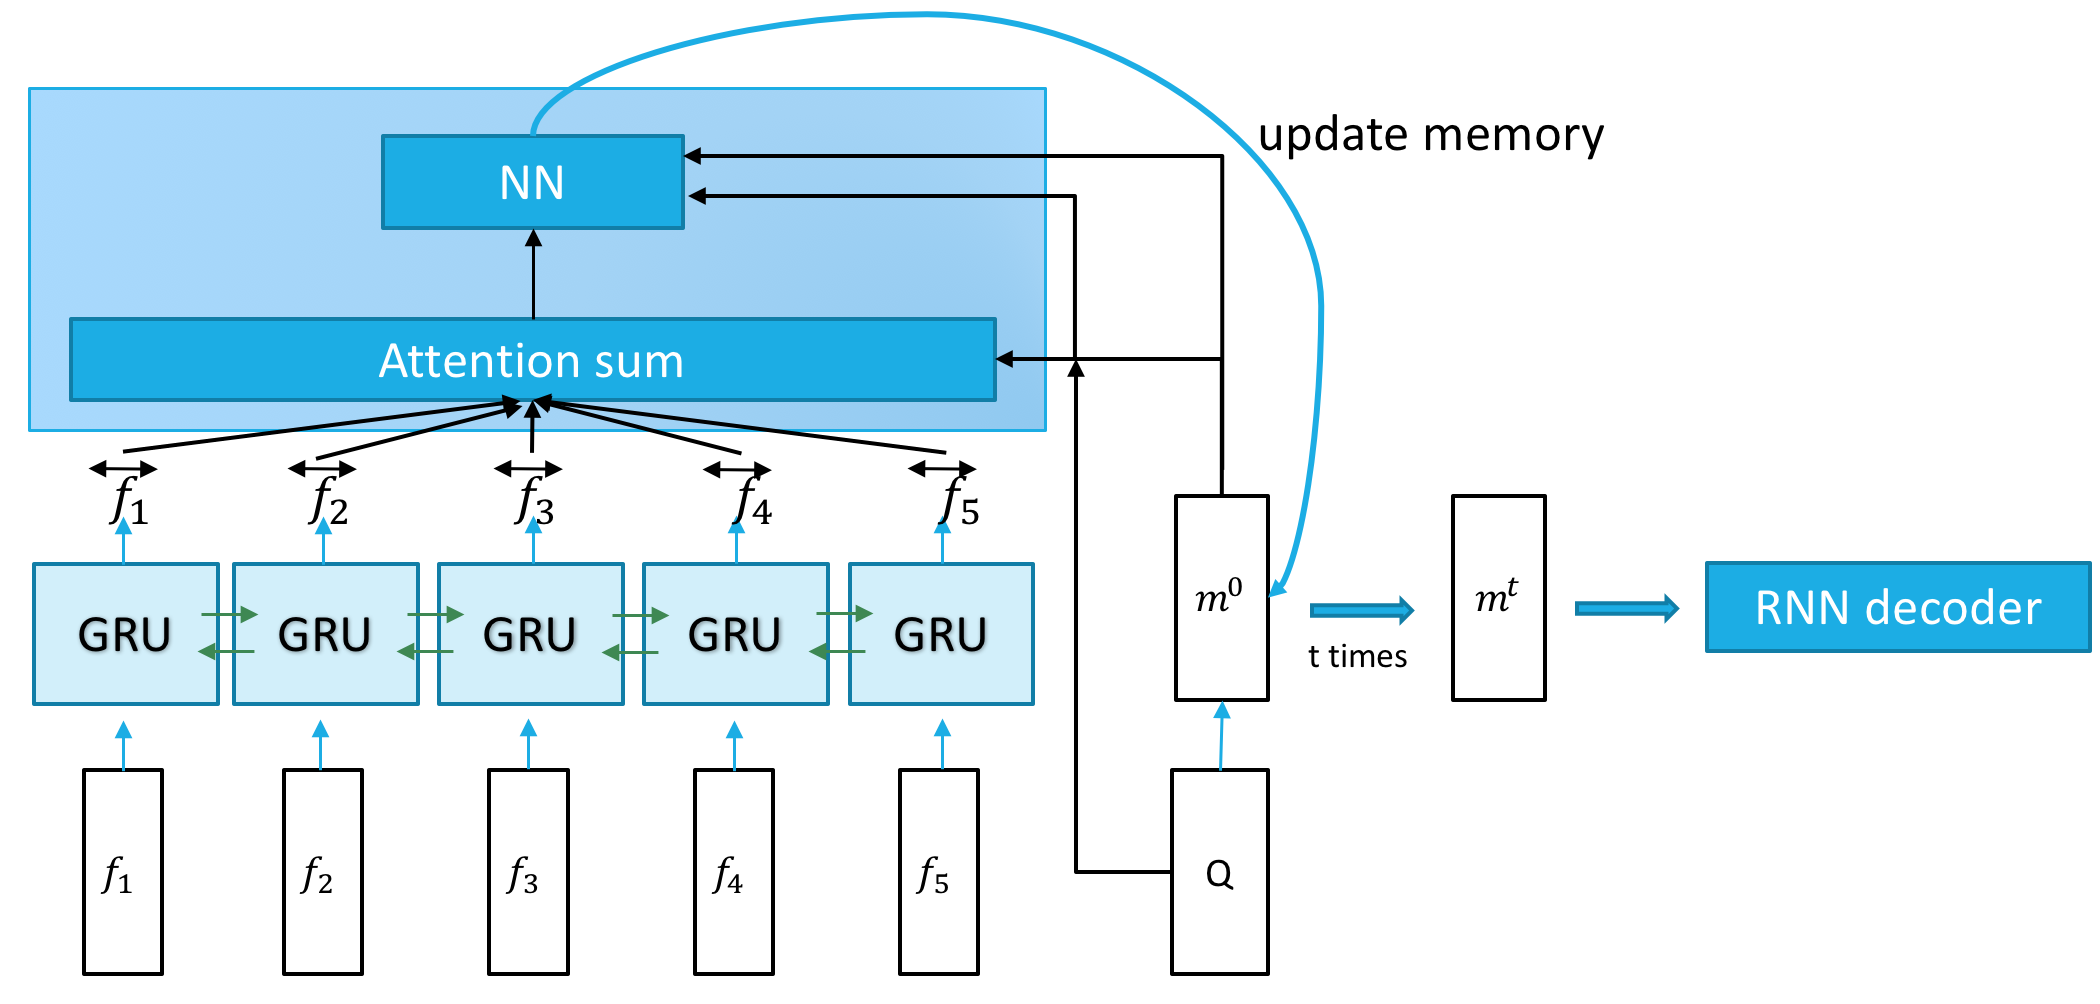
\includegraphics[scale=0.54]{images/chap3_dmn.png}
    \caption{專注式記憶編碼解碼器}\label{fig:dmn}
\end{figure}
\subsubsection{雙向式遞迴式類神經網路}
在得到句向量 $f_i$ 後,為了強化句子與句子彼此之間的關聯性,我們採取了雙向式遞迴式類神經網路(Bidirectional Recurrent Neural Network, BRNN),是由兩個遞迴式類神經網路,一為正向(Forward)遞迴式類神經網路輸出向量表示 $\overrightarrow{f_i}$ ,另一為反向(Backward)遞迴式類神經網路輸出向量表示 $\overleftarrow{f_i}$ ,並且取正向遞迴式類神經網路的第 $i$ 個時間點輸出向量 $\overrightarrow{f_i}$ ,與反向遞迴式類神經網路的第 $i$ 個時間點 $\overleftarrow{f_{M-i}}$ ,並把他們相加起來作為每個句子的向量表示 $\overleftrightarrow{f_i} = \overrightarrow{f_i} + \overleftarrow{f_i}$ ,即為圖(\ref{fig:dmn})中 GRU 之輸出。雖然採取了雙向式遞迴式類神經網路,但依然容易失去長期的資訊,且我們不僅僅只是要讀過文本而已,我們更需要結合查詢詞來回答問題,因此在此處我們導入了專注式機制(Attention Mechanism)的技術。

\subsubsection{專注式機制}
專注式的機制,就是為了比較查詢詞 $Q$ 與文本 $\overleftrightarrow{f_i}$ 之間的相關性,然而專注式機制的實作方法有很多,但核心的概念是為了找尋兩者間之相似性(Similarity),即稱為專注式權重 $\alpha_i$ ,以下是幾種常見計算專注式權重之方法:
\itemsep -4pt
\begin{itemize}
    \item 歐式距離:$\alpha_i = ||Q-\overleftrightarrow{f_i}||_{2}$
    \item 餘弦相似性:
            $\alpha_i = \frac{Q \circ \overleftrightarrow{f_i} }{|Q| |\overleftrightarrow{f_i}| } $ 
            ,其中 $\circ$ 為 逐點乘積
    \item 類神經網路: $\alpha_i = W_a ([Q ; \overleftrightarrow{f_i}]) $ 
        ,其中 $\alpha_i$ 為一純量(Scalar) $;$ 代表串連兩個向量。
\end{itemize}
本論文採取最後一種深度類神經網路的方法,然此處深度神經網路的輸入是為 $z_i$ ,結合句子 $\overleftrightarrow{f_i}$ 、問句 $Q$ 以及記憶 $m$ 表示的資訊,如式子($\ref{function:nninput}$)
\begin{equation}
    z_i = [ \overleftrightarrow{f_i} \circ Q ; \overleftrightarrow{f_i} \circ m ; |\overleftrightarrow{f_i} - Q| ; | \overleftrightarrow{f_i} - m| ] \label{function:nninput}
\end{equation}
其中 $m$ 是經由 $Q$ 來初始化,而 $|\cdot|$ 是向量取絕對值。

接著我們讓 $z_i$ 通過兩層類神經網路,可得一純量 $Z_i$。在得到了專注式權重 $Z_i$ 以後,我們對其做正規化,此處我們選擇「對所有句子的 $\alpha$ 值通過軟性最大化」,通過軟性最大化可以更加強化相關的句子,降低其餘句子的雜訊,如式子($\ref{function:attention}$)。
\begin{equation}
    g_i = \frac{exp{(Z_i)}}{\sum_{k=1}^{M} exp(Z_i)} \label{function:attention}
\end{equation}

結合正規化後的專注式權重 $g_i$ ,我們可對於文章抽取出基於我們想要專注點的語境向量(Contextual Vector),如式子(\ref{function:context_vector})。
%TODO contextual vector 中文
\begin{equation}
    c = \sum_{i=1}^{M} g_i \overleftrightarrow{f_i} \label{function:context_vector}
\end{equation}
%在得到了專注式權重以後,我們需要對其做正規化,
%而本篇論文另外使用了一種計算相似性的方法,
%\itemsep -2pt
%\begin{itemize}
%    \item Stochastic "Hard" Attention
%    \item Deterministic "Soft" Attention
%\end{itemize}
\subsubsection{記憶(Memory)}
在得到語境向量後,下一步則是要更新記憶 $m$ ,與計算專注式的權重一樣,通過一個類神經網路,輸入為當前的記憶、語境向量、以及固定的問句表示,進而更新記憶,如式子(\ref{function:update_memory})。
\begin{equation}
    m = ReLU(W [m; c; Q] +b) \label{function:update_memory}
\end{equation}
\subsubsection{回顧式機制}
在此,我們把計算專注式權重的值以及更新記憶的值,視為一個循環,我們把它稱為一個回顧,每經過一次回顧,相當於是再次讀過句子,重新理解再存入記憶裡,如圖(\ref{fig:dmn})所示,可以更新 t 次。
\subsubsection{解碼器}
最後再用儲存的記憶連接到一個遞迴式類神經網路,以便解碼出可能的答案,如式子 \ref{function:answer_module} ,而損失函數則是每個字的交叉熵。
\begin{equation}
    \label{function:answer_module}
    \begin{aligned}
    a_0 = m \\
    a_t = GRU(y_{t-1}, a_{t-1}) \\
    y_t = softmax(W^{(a)} a_t)
    \end{aligned}
\end{equation}

\section{基本實驗配置}
\subsection{前置處理}
\itemsep -4pt
\begin{itemize}
    \item 前處理:此數據集包含大量的英文,夾雜部分日文以及標點符號,若是選用所有的詞彙(Vocabulary),會有四十幾萬的詞(Word),我們試著降低詞彙的數量,移除掉標點符號和文本中的網址,並把所有英文字母轉成小寫,最後我們把詞彙量降到了約莫 14 萬個詞。
    \item 訓練方法:我們選擇將詞嵌入一併與我們的模型一起訓練。而為了避免過度貼合,對於所有的遞迴式類神經網路,都使用了丟棄演算法,而對於所有的可訓練的(Trainable)權重進行正規化。在回顧機制裡,我們設置回顧次數的範圍在 1 到 3 次。此外我們採用負採樣(Negative Sampling)的技巧,來降低整個模型所需要的參數量。
    \item 衡量標準:本論文對於問答系統所使用的衡量標準是 ROUGE (Recall-Oriented Understudy for Gisting Evaluation)\cite{lin2004rouge} ,常用於摘要(Summarization)或機器翻譯,是一種評比參考(Reference)字串和預測(Prediction)字串之間相似程度的量表,包含基於正確 n-元語法(n-gram)的 ROUGE-1 和 ROUGE-2 ,以及基於最長共同子字串(Longest Common Subsequence)長度的 ROUGE-L。ROUGE 值是一個介於 0 至 1 之間的實數,ROUGE 值表示兩字串的相似度越高。本篇論文採用的是 ROUGE-L 的分數。

\end{itemize}
\subsection{基準實驗}
我們總共提出兩種基準實驗模型,如圖(\ref{fig:baseline1})及(\ref{fig:baseline2})。
圖(\ref{fig:baseline1})先以問句當作編碼器的初始狀態,再將文本依序編碼,再用解碼器產生文字。圖(\ref{fig:baseline2})則是每個句子都和問句串接一起接到編碼器,之後再用解碼器產生文字。兩者的解碼器皆有使用 \cite{bahdanau2014neural} 專注式的技巧。
%TODO describe baseline
\begin{figure}[h]
    \centering
    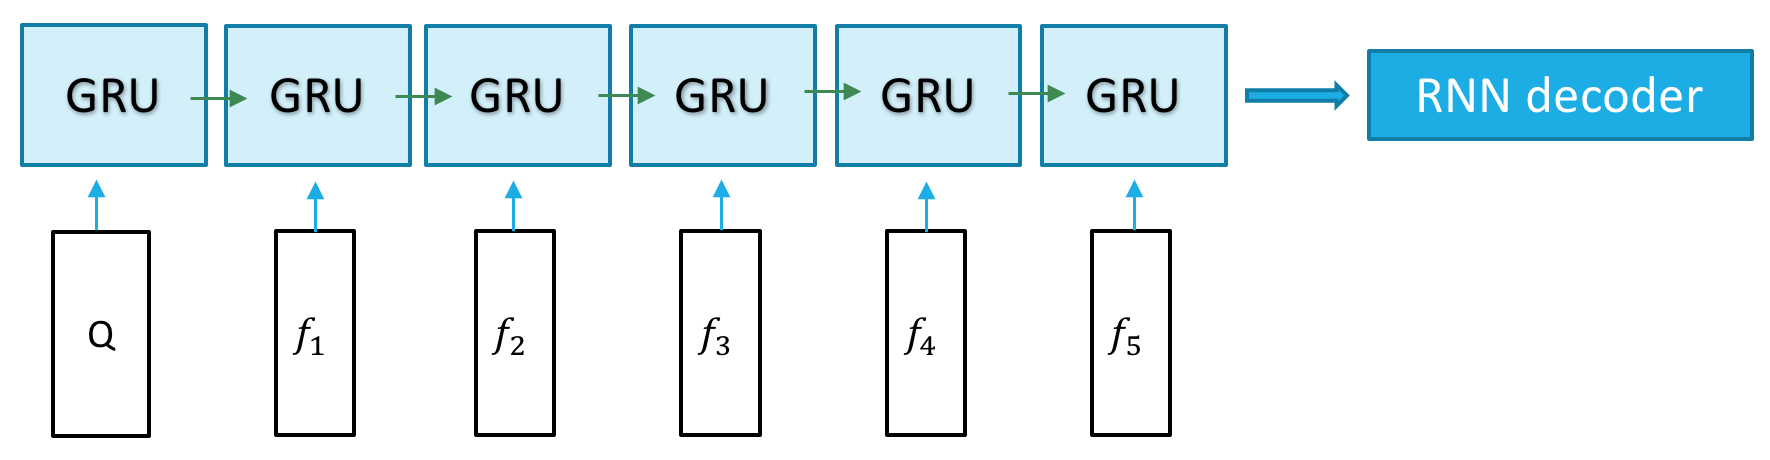
\includegraphics[scale=0.54]{images/chap3_baseline1.png}
    \caption{基準實驗模型一}\label{fig:baseline1}
\end{figure}
\begin{figure}[h]
    \centering
    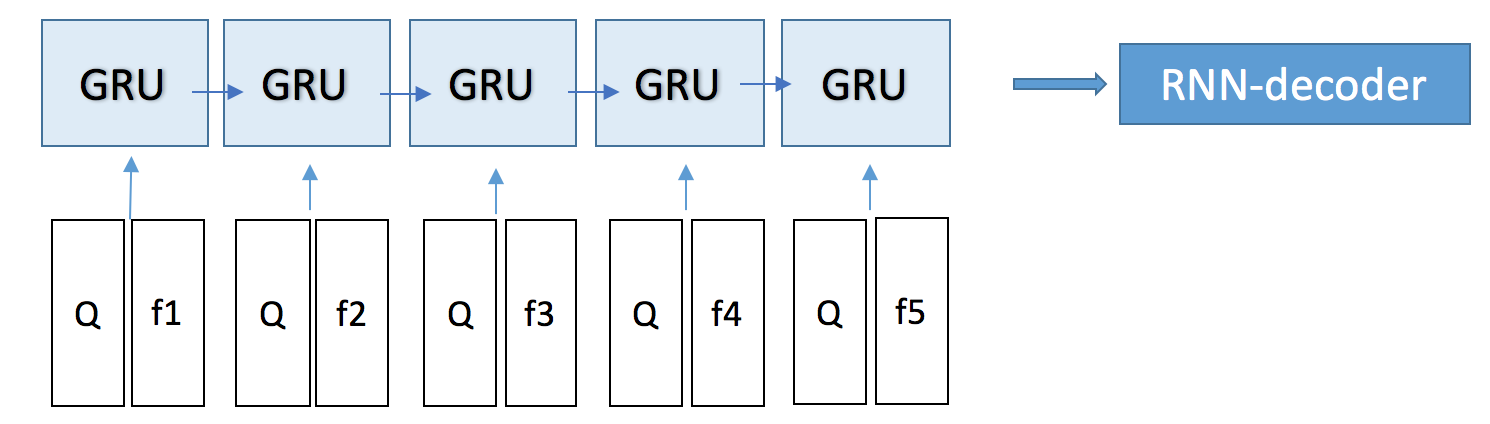
\includegraphics[scale=0.54]{images/chap3_baseline2.png}
    \caption{基準實驗模型二}\label{fig:baseline2}
\end{figure}

\section{實驗結果與討論}
\subsection{記憶細胞大小}
我們分別測試遞迴式網路的大小,分別是 128 、 256 以及 512 ,並試著增加詞向量的空間至 1000 維。
\begin{table}
    \caption{遞迴類神經網路實驗結果}
    \label{table:RNNCell_size}
    \centering
    \begin{tabular}{|l|l|l|}
        \hline
        記憶細胞大小&詞向量 & ROUGE\\
        \hline
        128 & 500 & 33.34\% \\ %Valkyrie\_0 \\
        \hline
        256 & 500 & 33.30\% \\
        \hline
        512 & 500 & 33.95\% \\
        \hline
        512 & 1000 & 33.22\% \\
        \hline
    \end{tabular}
\end{table}
\subsection{回顧次數}
我們在此測試回顧次數對模型之影響的影響。如表 \ref{table:hop} 可見,最佳的情況是發生在兩次的情形。%可能不需要太多次的回顧,甚至有些語意只需要一次便能理解。
\begin{table}
    \caption{回顧次數實驗結果}
    \label{table:hop}
    \centering
    \begin{tabular}{|l|l|}
        \hline
        回顧次數 & ROUGE\\
        \hline
        1 & 33.63\% \\
        \hline
        2 & 33.95\% \\%34426306Valkyrie\_1\\
        \hline
        3 & 33.22\% \\
        \hline
    \end{tabular}
\end{table}
\subsection{取代數字}
另外,為了再降低複雜度,我們特別對阿拉伯數字進行處理,把所有阿拉伯數字取代成特定標籤,或者是以文本數字出現的順序,分別給予數字一、數字二、數字三等等,把詞彙量降低到 13 萬左右。
\begin{table}
    \caption{數字處理}
    \label{table:digit}
    \centering
    \begin{tabular}{|l|l|}
        \hline
        數字取代方法 & ROUGE\\
        \hline
        保留數字 & 24.13\% \\%Caishen\_1 \\
        \hline
        統一所有數字 & 33.68\% \\
        \hline
        數字依文章順序標注 & 33.95\% \\
        \hline
    \end{tabular}
\end{table}
\subsection{模型比較}
由表 \ref{table:model} 可見,基準實驗模型的表現只有 20\% 左右,我們的模型相較之下大幅領先。然而,雖然目前仍無法到達人類的標準,但相信對於問答系統已經是一大突破了。
\begin{table}
    \caption{模型比較}
    \label{table:model}
    \centering
    \begin{tabular}{|l|l|}
        \hline
        模型 & ROUGE\\
        \hline
        基準實驗模型一 & 18.63\% \\
        \hline
        基準實驗模型二 & 22.01\% \\%Venus\_0 \\
        \hline
        ReasoNet Baseline \cite{shen2016reasonet}& 19.20\% \\
        \hline
        FastQA \cite{weissenborn2017making} &32.09\% \\
        \hline
        專注式記憶編碼解碼器 &  33.95\% \\ %best\_score
        \hline
        Human Performance &47\% \\ %TODO 中文
        \hline
    \end{tabular}
\end{table}
%\subsection{更新記憶方法}
\section{範例與分析}
我們挑選幾個專注式機制在不同回顧的次數所專注之表現,如圖 \ref{fig:attn_1} 、 \ref{fig:attn_2} 和圖\ref{fig:attn_3}。

圖 \ref{fig:attn_1} 的問句為「how many years to become an accountant」,答案為「Four year」,與我們模型產生的句子結果一樣。而看圖可發現回顧三次可以會越來越集中於含有標準答案資訊的句子。再看
圖 \ref{fig:attn_2} ,其問句為「what region is indiana in」,答案為「U.S」,而我們模型產生的是「north county」,雖專注的點正確了,但卻與答案不同,僅僅對了部分的意思,並未提及美國相關的詞,我們進一步觀察到在其他訓練階段所產生的句子有「united states」、「north america」跟「us」等,由此可見,模型應該有學習到答案是「美國」相關的意思。
\begin{figure}
    \centering
    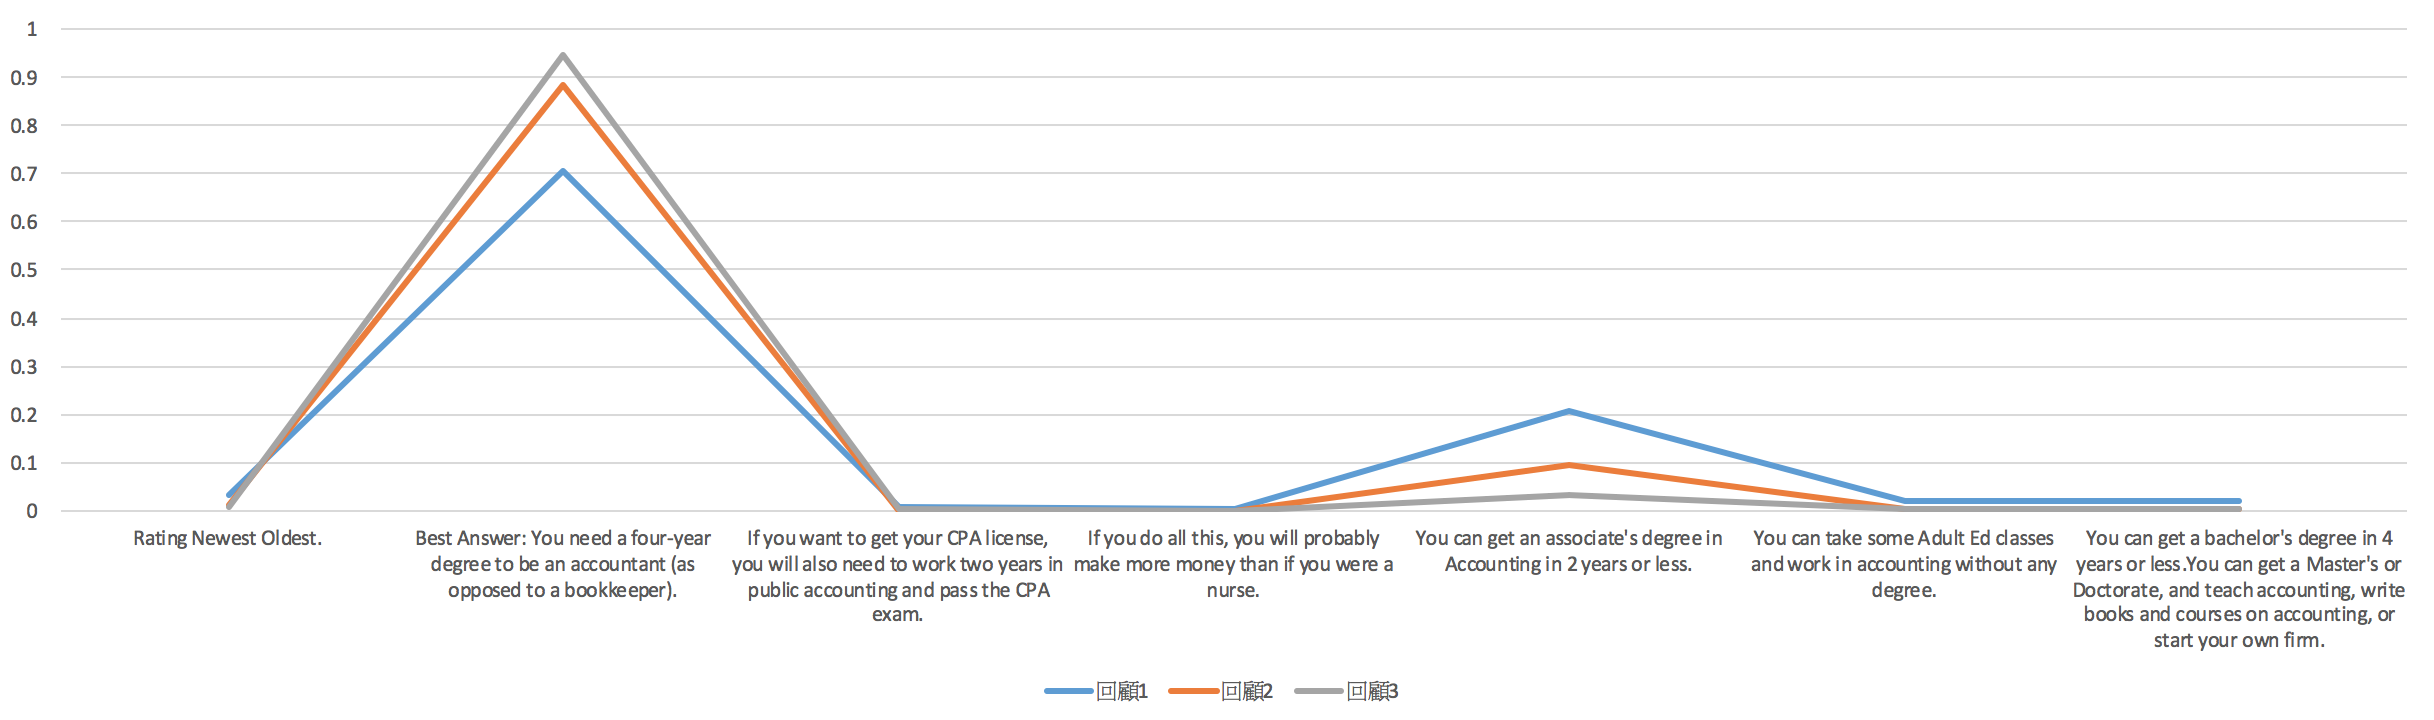
\includegraphics[scale=0.55,angle=90]{images/chap3_attn1.png}
    \caption{專注式結果1}\label{fig:attn_1}
\end{figure}
\begin{figure}
    \centering
    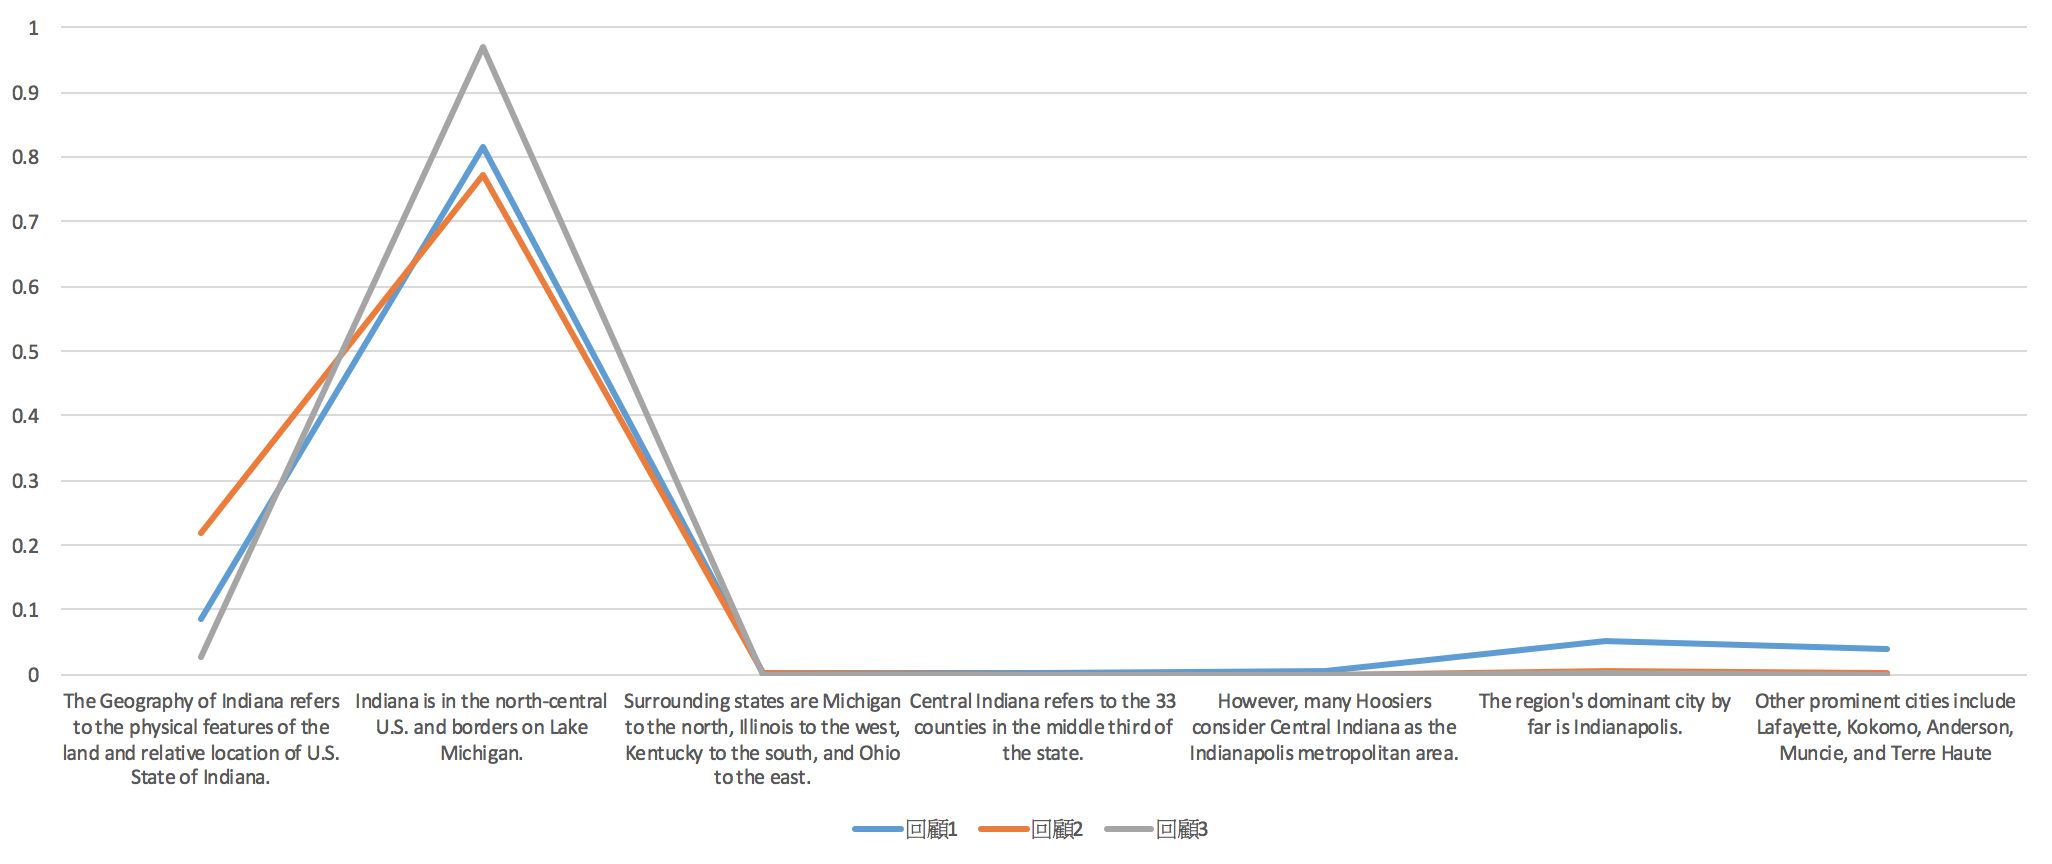
\includegraphics[scale=0.58,angle=90]{images/chap3_attn2.png}
    \caption{專注式結果2}\label{fig:attn_2}
\end{figure}

圖 \ref{fig:attn_3} 為一反例,其問句為「what means irie」,答案是「Alright, powerful and pleasing, excellent, highest, the state of feeling great.」,而我們模型所生成之答案為「comfort」,並無與答案完全一樣的字詞,且其專注點位於第一句「Irie (I rie I '  ree) is the word in Jamaican Patois that means, alright.」,而以我們人類角度來看,與答案有相關的應為第二句「The term can be used to mean 1: powerful and pleasing; 2: excellent, highest; n 3: the state of feeling great.」。
\begin{figure}
    \centering
    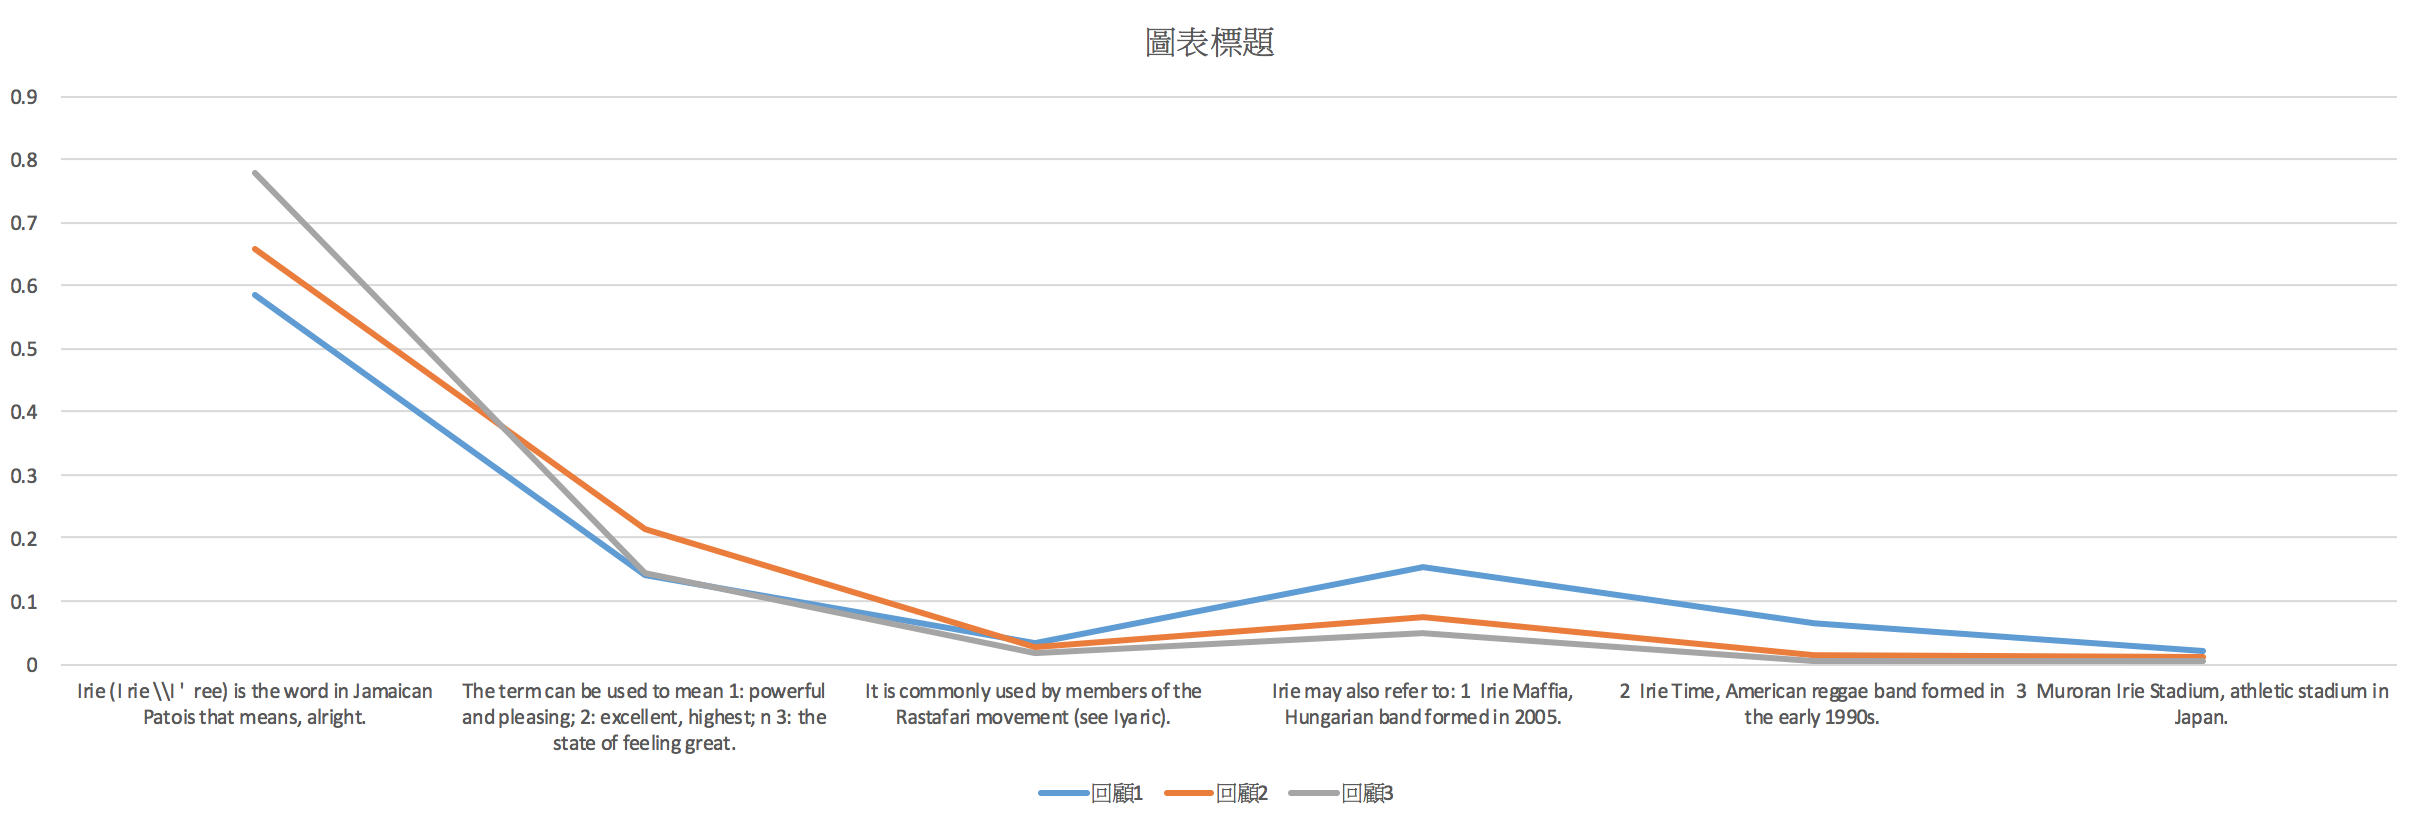
\includegraphics[scale=0.55,angle=90]{images/chap3_attn4.png}
    \caption{專注式結果3}\label{fig:attn_3}
\end{figure}

%TODO analysis weight
\begin{figure}
\end{figure}
\section{本章總結}
在本章節我們試著針對問句與其對應之文本,來產生可能之答案,可見我們在有限制領域裡,已經能有不錯的表現,達到 33.95 \% 。然而,要能夠回答更廣泛的問題,我們需要有效的方法,找出可能含有答案的文本,這部分我們將在第四章介紹。另外,我們發現對於要回答過長的句子,失真的可能性相當高,對此解決方法,我們將在第五章介紹。
%從實驗當中可以發現,我們已經不難從單一文本之中產生答案,然而
%雖然機器可以回答出部分的正確問題,但在此處我們是基於特定文本,以期望機器給予正確回答,但現實情況中,我們必須基於大量的資訊,因此我們要試著從大量的資訊中挑選出相關的文本,能使我們的模型更加有用。
